%!TEX root = main.tex

\subsection{What is a corpus ?}

A large body of linguistic evidence typically composed of attested language use.

There is several desired characteristics of a corpus:
\begin{itemize}
	\item Machine readable;
	\item Sampled (aiming at balance and representativeness);
	\item Well-organized and formatted;
	\item Big.
\end{itemize}

\subsubsection{Whats is a corpus for ?}

\begin{itemize}
	\item For linguists:
	\begin{itemize}
		\item Empirical approach (based on facts)
		\item Chomsky does not like it because it captures bits of performance but not competence. 
	\end{itemize}
	\item In NLP: the raw fuel of NLP.
\end{itemize}

\subsubsection{Typology}

There is two category of corpus: \textbf{monolingual} and \textbf{multilingual}. The first one has three types:
\begin{itemize}
	\item \textbf{Reference corpus}: large, balanced and \textit{representative}, it is designed to provide comprehensive information about a language;
	\item \textbf{Specialized corpus}: corpus designed to cover one particular aspect of the language;
	\item \textbf{Static} vs. \textbf{Monitor corpus}: Static corpus does not evolve.
\end{itemize}

The second one (\textbf{multilingual}) has two types:
\begin{itemize}
	\item \textbf{Comparable corpora}: several corpora of various languages collected using the same sampling method and similar balance in order to permit comparisons between corpora;
	\item \textbf{Parallel corpora}: gather a corpus in one language and the translation of this corpus in one or more orther languages.
\end{itemize}

\subsubsection{Collection}

\textbf{Oral corpora} are collected from recordings of interview, conferences, radio or TV programs, \dots \textbf{Written corpora} are collected from digitalization of analogical sources, digital sources, web, \dots

\subsection{Corpus Annotation}

The aim of corpus annotation is to make explicit some linguistic infor- mation that is part of the text. This is done by adding metadata to the text. Automatic or manual.

There is 6 levels of annotations:
\begin{itemize}
	\item morpho-syntactic annotation;
	\item lemmatization;
	\item syntactic annotation (treebanks);
	\item semantic annotation (entities, word meaning, predicates, etc.);
	\item discourse annotation (ie: anaphora);
	\item phonetic transcription.
\end{itemize}

\begin{figure}[htp]
	\centering
	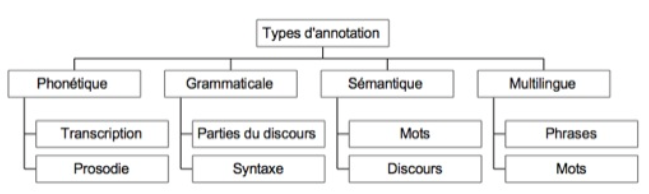
\includegraphics[scale=0.6]{images/07_levels.png}
 	\caption{Levels of annotation.}
\end{figure}

There is some standards for annotation: the goal is to ensure corpora \textbf{reusability} and software \textbf{interoperability}.

\subsection{Corpus Processing}

Here is the typical steps of corpus processing:
\begin{itemize}
	\item \textbf{Text formatting and normalization}
	\item \textbf{Tokenization}: Sevral ways to do it. Type/Token Ratio.
	\item \textbf{Lexical analysis}
	\begin{itemize}
		\item \textbf{Morphological analysis}: Based on dictionary and morphological rules. On the fly and can process new words. If only dictionary based, it is quick but limited on the dictionary coverage.
		\item \textbf{POS tagging}: Remove ambiguity (walk: noun or verb ?)
		\item \textbf{Lemmatization}
	\end{itemize}
	\item \textbf{Entitites recognition}
	\item \textbf{Syntactic analysis}
	\item \dots
\end{itemize}
